\chapter{Method}\label{sect:method}


\fancyfoot[RE,LO]{2. METHOD}

\Cref{fig:hesse} depicts the powerset of all possible worlds in a $3$-dimensional system. In the models that follow, an agent's opinion is given by its distribution of probabilities over each of these possible worlds, shown as singleton sets in the diagram. Hence, the set of beliefs held by the $i^\textnormal{th}$ agent can be represented by the vector

\begin{center}
$ \underline{\mathbf{P}}^t_i = \begin{bmatrix}
    p_{i, 1}\\
    p_{i, 2}\\
    p_{i, 3}
\end{bmatrix}$,
\end{center}

where $p_{i,j}$ is the probability value that the $i^\textnormal{th}$ agent has placed in state $\{H_j\}$. By the axiom $P(\mathbf{W}) = 1$, the vector $\underline{\mathbf{P}}^t_i$ must also sum to $1$. This allows us to form a right-stochastic matrix\footnote{A right stochastic matrix is defined as a square, non-negative matrix for which the rows sum to $1$~\cite{Gagniuc2017MarkovExperimentation}.} representing the collective beliefs of $K$ agents over $n$ states of the world at time $t$,

\begin{center}
$\underline{\underline{\mathbf{P}}}^t = \begin{bmatrix}
    p_{1, 1} & p_{1, 2} & p_{1, 3} & \dots  & p_{1, n} \\
    p_{2, 1} & p_{2, 2} & p_{2, 3} & \dots  & p_{2, n} \\
    \vdots & \vdots & \vdots & \ddots & \vdots \\
    p_{K, 1} & p_{K, 2} & p_{K, 3} & \dots  & p_{K, n}
\end{bmatrix}$.
\end{center}

Each of the $K$ agents is initialised with $n$ distinct beliefs computed using \cref{alg:initialise}. In a $3$-dimensional case, agents' beliefs can be represented as a point on the blue surface shown in~\cref{fig:3d-simplex}, referred to as a simplex. This surface can be projected down to a $2$-dimensional plot, shown in~\cref{fig:2d-simplex}, referred to as a Barycenter plot. In this plot, an agent in the corner of the triangle is described as being certain, extremist, or having a strong belief in a single hypothesis. Conversely, an agent with uncertain or weak beliefs holds an approximately uniform distribution and so is found in the central region of Barycentric space.

\begin{algorithm}[H]
\SetAlgoLined
\KwResult{Initialisation of the beliefs of $K$ agents }
 \While{$i < K$}{
  $d \gets drawRandomNumbers(n-1)$\;
  $d \gets sort(d)$\;
  $prepend(0, d); append(1,d)$\;
  $beliefs \gets consecutiveElementwiseDifference(d)$;  \hspace{1em} \textit{$\triangleright$ returns list $(j+1)^\textnormal{th}$ - $j^\textnormal{th}$ values}\\
  $i++$\;
 }
 \caption{Agent Initialisation}
 \label{alg:initialise}
\end{algorithm}












\begin{figure}[H]
\begin{minipage}[ht]{0.45\textwidth}
    \centering
    \resizebox{\linewidth}{0.74\linewidth}{
   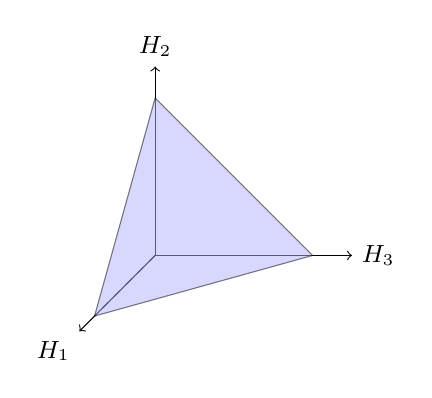
\begin{tikzpicture}[line join = round, line cap = round]
\coordinate [] (A) at (2,0,0);
\coordinate [] (B) at (0,0,2);
\coordinate [] (C) at (0,2,0);
\coordinate [] (D) at (0,0,0);

\draw[->] (0,0) -- (2.5,0,0) node[right] {\small $H_3$};
\draw[->] (0,0) -- (0,2.4,0) node[above] {\small $H_2$};
\draw[->] (0,0) -- (0,0,2.5) node[below left] {\small $H_1$};
\foreach \i in {A,B,C,D}
    \draw[dashed] (0,0)--(\i);
\draw[-, fill=blue!30, opacity=.5] (A)--(B)--(C)--cycle;
\end{tikzpicture} }
\subcaption{$3$-dimensional simplex}\label{fig:3d-simplex}
\end{minipage}
\hfill
  \begin{minipage}[ht]{0.45\textwidth}
    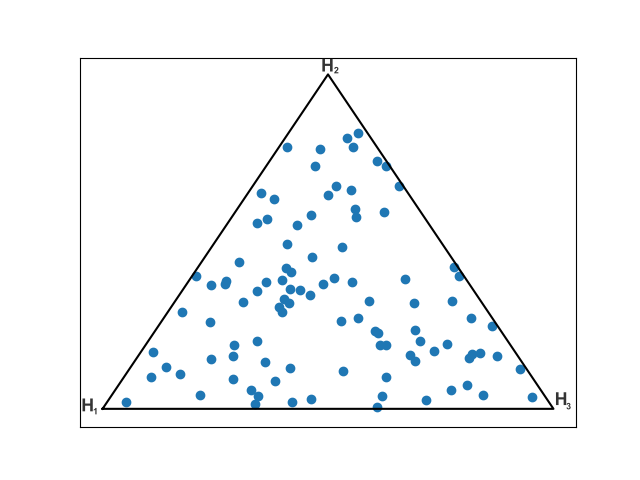
\includegraphics[width=\textwidth]{Images/Figures/Barycenter/ExampleBarycentre.png}
    \subcaption{$2$-dimensional projection}\label{fig:2d-simplex}
 \end{minipage}
\caption{An example of a $3$-dimensional simplex over a world with $3$ possible states, projected down to $2$-dimensions, referred to as a Barycenter plot. } 
\end{figure}

Once the population is initialised, the communication protocols between agents must be defined, requiring a number of simplifications. One such simplification comes from Parker and Zhang, who describe a characteristic of their model which they name the ``well-stirred'' assumption. This assumes that the population is sufficiently mixed together that it is acceptable to select agents at random to communicate. The assumption can be thought of in a similar way to the social lattice described in~\cite{Deffuant2000MixingAgents}, though instead of a simple square lattice, the network is fully connected with communicating pairs selected at random. In \cref{fig:simple_interaction}, two agents are drawn randomly from the population, one to be the speaker, one to be the listener. This model is based on a special case of the signalling games introduced by~\cite{Lewis2002Convention:Study}. This work describes a communicator that acts in its best interests to convey a message that reflects a state of the world that it perceives to be true. The communicator then broadcasts its message to an audience who react to the information they receive. In our case, the audience is one agent, the listener, as shown in~\cref{fig:simple_interaction}. The communication created by the speaker is an argument it hopes will persuade the listener to update its beliefs to more closely align with the speaker's. 

 \begin{figure}[H]
 	\centering
 	\begin{tikzpicture}[
    ->,
    >=stealth',
    auto,
    semithick,
    node distance=3cm,
    state/.style={
        circle,
        draw,
    },
]
    \begin{scope}[
        every node/.append style={
            state,
        },
    ]
        \node (x0)                     {S};
        \node (x3) [right of=x0] {L};
    \end{scope}
    
    \path
    (x0) edge [loop above, looseness=10, in=100, out=160] node        {Create Assertion}  (x0)
         edge [bend left]                                 node [swap] {Send}              (x3)
    (x3) edge [loop above, looseness=10, in=80, out=20]   node        {Update}            (x3);
\end{tikzpicture}

 	\caption{Simple model of the interaction between two agents. \textit{S} is randomly selected each iteration as the speaker and \textit{L} is randomly selected each iteration as the listener. \textit{S} creates an argument that it transmits to \textit{L}. \textit{L} may then update its own beliefs according to the argument it receives from \textit{S}.}
 	\label{fig:simple_interaction}
 \end{figure}
 
Initially, it is assumed that the speaker is aware of the listener's opinions prior to making an assertion, as well as how the listener will react upon hearing it. \cref{alg:method} is run until either the maximum number of iterations is reached or the system can be said to have converged, as defined in~\cref{eq:convergence}. This is clearly a greatly simplified interaction, and is therefore not equivalent to any human conversation, no matter how simplistic. However, it serves as an approximate model, allowing the behaviour of the population to be studied in a framework that is explainable. 


\begin{algorithm}[H]
\SetAlgoLined
\KwResult{Simulation of agent based communication }
 initialisation\;
 \While{$t < t_{max}$}{
  selectSpeaker\;
  selectListener\;
  speakerConstructArgument\;
  listenerReactToArgument\;
  \eIf{converged}{
   break\;
   }{
   t++\;
  }
 }
 \caption{Method}
 \label{alg:method}
\end{algorithm}

There are several useful metrics for describing the dynamics of this system. The average entropy of the population as a whole gives the level to which the agents have become certain in a single state~\cite{Shannon1948ACommunication}. This is defined as

\begin{equation}\label{eq:shannon_entropy}
    \hat{E}^t = \frac{1}{K} \sum_i^K - \underline{\mathbf{P}}^t_i \cdot \log ( \underline{\mathbf{P}}^t_i).
\end{equation}

The system is said to have converged when the entropy has not changed by more than $\eta $ for $T$ iterations, expressed as 

\begin{equation}\label{eq:convergence}
    \Delta \hat{E}^T = \abs{ \hat{E}^t -  \hat{E}^{t+T}}  \leq \eta. 
\end{equation}

However, entropy only highlights whether the agents hold strong beliefs, not that they agree on those beliefs. Hence, the J-Divergence is used as a symmetric version of KL-Divergence, to determine the average distance between all pairs of agents $(i,k)$ in probability space~\cite{Johnson2001SymmetrizingDistance}. It is defined as

\begin{equation}
    \hat{J}^{t} = \frac{1}{K} \sum_k^K \frac{1}{K} \sum_i^K  \frac{1}{2} \left( \underline{\mathbf{P}}^t_i \log \left( \frac{ \frac{1}{2} (\underline{\mathbf{P}}^t_i + \underline{\mathbf{P}}^t_k) }{\underline{\mathbf{P}}^t_i} \right) +  \underline{\mathbf{P}}^t_k \log \left( \frac{ \frac{1}{2} (\underline{\mathbf{P}}^t_i + \underline{\mathbf{P}}^t_k) }{\underline{\mathbf{P}}^t_k} \right) \right).
\end{equation}

The two aspects of~\cref{fig:simple_interaction} are the creation of the speaker's assertion and the response of the listener. For the former, four models are proposed ranging from simply broadcasting the speaker's beliefs to tailoring the argument to the listener. For the latter, four models are defined describing different behaviours the listeners can adopt. These include the listener reacting passively, with discernment, or with steadily less and less importance placed on new information as time passes.







